\setlength{\columnsep}{3pt}
\begin{flushleft}
	
	\begin{itemize}
		
		\item IP address consists of 2 parts:
		\begin{itemize}
			\item \textbf{Network bit}: Defines the network of your IP
			\item \textbf{Host bit} : Defines the IP address of your machine
		\end{itemize}
		\begin{figure}[h!]
			\centering
			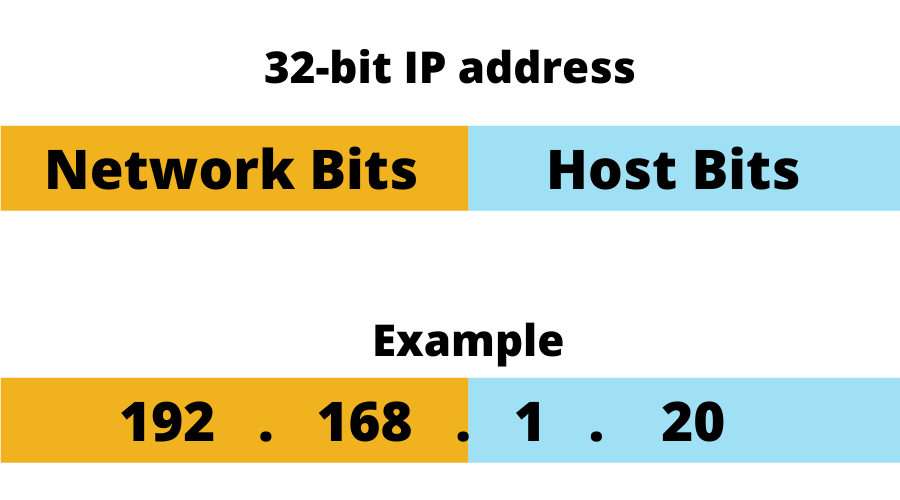
\includegraphics[scale=0.6]{content/chapter14/images/network_host.png}
			\caption{Network bit \& Host bit}
			\label{fig:network_host}
		\end{figure}
		\item \textbf{How do we decide what part of IP address is network bit \& host bit?}
		\item \textbf{Answer: Netmask}
		\newpage
	\end{itemize}
		
	
\end{flushleft}
\newpage


